
%%%%%%%%%%%%%%%%                                ~~~~~~~~~~~~~~~~~~~~~~~~~~~~~~~~~~~~~~~~~~~~~~~~~~
% CONDITIONALS %
%%%%%%%%%%%%%%%%                                ~~~~~~~~~~~~~~~~~~~~~~~~~~~~~~~~~~~~~~~~~~~~~~~~~~

\newif\ifPeerReview\PeerReviewfalse             % Whether to create the PeerReview version or
                                                % Journal version
\newif\ifFlatArchive\FlatArchivefalse           % Whether archive is flat (messy) or contain 
                                                % subfolders for graphics etc.
\newif\ifFloatAtEnd\FloatAtEndfalse             % Available in PeerReview mode:
                                                % Place floats at end of document?
\newif\ifTODO\TODOtrue                          % Use todo notes?

%%%%%%%%%%%%%%                                  ~~~~~~~~~~~~~~~~~~~~~~~~~~~~~~~~~~~~~~~~~~~~~~~~~~
% ECUA style %
%%%%%%%%%%%%%%                                  ~~~~~~~~~~~~~~~~~~~~~~~~~~~~~~~~~~~~~~~~~~~~~~~~~~

\documentclass[10pt,a4paper]{article}
\usepackage{template/ecua}

%%%%%%%%%%%%%%%%%%%%%%%%%%%%%%                  ~~~~~~~~~~~~~~~~~~~~~~~~~~~~~~~~~~~~~~~~~~~~~~~~~~
% ECUA ''APPROVED'' PACKAGES %
%%%%%%%%%%%%%%%%%%%%%%%%%%%%%%                  ~~~~~~~~~~~~~~~~~~~~~~~~~~~~~~~~~~~~~~~~~~~~~~~~~~

% load some other useful packages
\usepackage{cite} % improved formatting for citation lists
\usepackage{graphicx}

%%%%%%%%%%%%%%%%%%%%%%%                         ~~~~~~~~~~~~~~~~~~~~~~~~~~~~~~~~~~~~~~~~~~~~~~~~~~
% ADDITIONAL PACKAGES %       
%%%%%%%%%%%%%%%%%%%%%%%                         ~~~~~~~~~~~~~~~~~~~~~~~~~~~~~~~~~~~~~~~~~~~~~~~~~~

\usepackage{glossaries}
\usepackage[table,dvipsnames,svgnames]{xcolor}
\newcounter{todoidx}

\ifTODO
   \definecolor{todobackground}{rgb}{0.95,0.95,0.95}
   \setlength\marginparsep{1pt}
   \setlength\marginparwidth{35pt}
   \newlength\marginparwidthsmall
   \setlength\marginparwidthsmall{\marginparwidth}
   \addtolength\marginparwidthsmall{+6mm}
   \newcommand\todo[1]{%
      \addtocounter{todoidx}{1}%
      {\color{Red}\fbox{\bf\thetodoidx{}}}%
      \marginpar{%
         {\vspace*{-10pt}\color{Red}\fbox{\bf\thetodoidx{}}}\\%
         \fcolorbox{red}{todobackground}{\parbox{\marginparwidthsmall}{\scriptsize #1}}}}

   \newcommand\todopar[1]{\fcolorbox{red}{white}{\parbox{0.97\linewidth}{#1}}}
\else
%    \usepackage[disable]{./todonotes} 
   \newcommand\todo[1]{}
\fi

\newenvironment{narrow}[2]{%
\begin{list}{}{%
\setlength{\topsep}{0pt}%
\setlength{\leftmargin}{#1}%
\setlength{\rightmargin}{#2}%
\setlength{\listparindent}{\parindent}%
\setlength{\itemindent}{\parindent}%
\setlength{\parsep}{\parskip}}%
\item[]}{\end{list}}

\usepackage{float}

%%%%%%%%%%                                      ~~~~~~~~~~~~~~~~~~~~~~~~~~~~~~~~~~~~~~~~~~~~~~~~~~
% MACROS %       
%%%%%%%%%%                                      ~~~~~~~~~~~~~~~~~~~~~~~~~~~~~~~~~~~~~~~~~~~~~~~~~~


\newcommand\Grey[1]{{\color{Grey}#1}}
\newcommand\Red[1]{{\color{Red}#1}}
\newcommand\Blue[1]{{\color{Blue}#1}}
\newcommand\DarkBlue[1]{{\color{DarkBlue}#1}}
\newcommand\LightBlue[1]{{\color{LightBlue}#1}}
\newcommand\Brown[1]{{\color{Brown}#1}}
\newcommand\Green[1]{{\color{Green}#1}}
\newcommand\SeaGreen[1]{{\color{SeaGreen}#1}}
\newcommand\Yellow[1]{{\color{yellow}#1}}
\newcommand\Orange[1]{{\color{orange}#1}}

\newcommand\nn{\nonumber\\}

\newcommand\nmat[1]{\begin{matrix}#1\end{matrix}}
\newcommand\bmat[1]{\begin{bmatrix}#1\end{bmatrix}}
\newcommand\case[1]{\begin{cases}#1\end{cases}}
\newcommand\textbox[2]{\footnotesize\text{\parbox{#1}{\centering\emph{#2}}}}

\newcommand\rand{\text{rand}}
\newcommand\randn{\text{randn}}
\newcommand\rect{\text{rect}}
\newcommand\sinc{\text{sinc}}
\newcommand\tr{\text{tr}}
\newcommand\adj{\text{adj}}

% \newcommand\max{\text{max}}
\newcommand\argmin{\text{argmin}}

\newcommand\qqquad{\quad\qquad}
\newcommand\qqqquad{\qquad\qquad}

\renewcommand\l[1]{\left#1}
\renewcommand\r[1]{\right#1}

% {\text{\parbox{1.5cm}{\centering volume hyper- sphere}}}

%Keyword colouring:
\newcommand\kw[1]{#1}
\newcommand\parm[1]{#1}%\color{Black}#1\color{Black}}

\newcommand\of[1]{\scriptstyle(\parm{#1})\displaystyle}
\newcommand\df[1]{\scriptstyle[\parm{#1}]\displaystyle}
\newcommand\var[3]{#1_\text{#2}\of{#3}}

\newcommand\diag{\text{diag}}

% \raisebox{lift}[extend-above-baseline][extend-below-baseline]{text}
\newcommand\mt[1]{\text{\emph{#1}}} %mt = mathtext
\newcommand\mathnorm{\textstyle}
\newcommand\mathbig[1]{\displaystyle#1\mathnorm}
\newcommand\mathsmall[1]{\scriptstyle#1\mathnorm}
\newcommand\mathtiny[1]{\scriptscriptstyle#1\mathnorm}
\newcommand\sfrac[2]{\scriptstyle\raisebox{0.25pt}[0pt][0pt]{$\frac{#1}{#2}$}\mathnorm}
\newcommand\nfrac[2]{\textstyle\frac{#1}{#2}\displaystyle}

\newcommand\sumu[1]{\sum\limits^{#1}\,}
\newcommand\suml[1]{\sum\limits_{#1}\,}
\newcommand\sumb[2]{\sum\limits_{#1}^{#2}\,}

\newcommand\produ[1]{\prod\limits^{#1}\,}
\newcommand\prodl[1]{\prod\limits_{#1}\,}
\newcommand\prodb[2]{\prod\limits_{#1}^{#2}\,}

\newcommand\defeq{\overset{\underset{\mathrm{def}}{}}{=}}

%Math macros:
\newcommand\diff[2]{\frac{\kw{d}\,\textstyle #1\scriptstyle}{\kw{d\parm{#2}}}\displaystyle}
\newcommand\ddiff[2]{\frac{\kw{d^2}\,\displaystyle #1\scriptstyle}{\kw{d\parm{#2}}^2}\displaystyle}

\renewcommand\d[1]{\scriptstyle\kw{\,d\parm{#1}}\displaystyle}

% These commands are mutually exclusive. Remember to "renew" in v2.
\newcommand\intb[4]{\int\limits_{#3}^{#4} #1 \d{#2}} % \int{exp}{var}{from}{to}
\newcommand\intl[3]{\int\limits_{#3} #1 \d{#2}} % \int{exp}{var}{for all}
\newcommand\intu[2]{\int #1 \d{#2}} % \int{exp}{var}{for all}

\newcommand\T{^{\scriptscriptstyle T}}
\renewcommand\H{^{\scriptscriptstyle H}}

\renewcommand\vec[1]{\boldsymbol{#1}}
\newcommand\mat[1]{\boldsymbol{#1}}

\newcommand\1{\vec 1}
\newcommand\I{\mat I}
\renewcommand*\a{\vec a}
\renewcommand*\i{\vec i}
\renewcommand*\k{\vec k}
\newcommand*\n{\vec n}
\newcommand*\p{\vec p}
\newcommand*\s{\vec s}
\newcommand*\w{\vec w}
\newcommand*\x{\vec x}
\newcommand*\y{\vec y}

\newcommand*\A{\mat A}
\newcommand*\B{\mat B}
\newcommand*\C{\mat C}
\newcommand*\E{\mat E}
% \renewcommand*\H{\mat H}
\renewcommand*\P{\mat P}
\newcommand*\eP{\mat{\hat P}}
\newcommand*\R{\mat R}
\newcommand*\Ri{\R^{-1}}
\newcommand*\eR{\mat{\hat R}}
\newcommand*\eRi{\hat{\mat R}\,\!^{-1}}
\newcommand*\Navg{N_\text{avg}}
\newcommand*\W{\mat W}
\newcommand*\X{\mat X}
\newcommand*\Xd{\X_{\!\Delta}}
\newcommand*\Y{\mat Y}

\renewcommand*\L{\mat \Lambda}
\newcommand*\U{\mat U}
% \renewcommand*\t{\mathtiny{^T}}
% \newcommand*\h{\mathtiny{^H}}
\renewcommand*\t{^T}
\newcommand*\h{^H}

\newcommand\D{\vec\nabla} %Del: Vector differential operator - nabla
\newcommand\Dx{\vec\nabla\times}
\newcommand\Dd{\vec\nabla\cdot}

\usepackage{tikz}
\usetikzlibrary{shapes,snakes}
\usepackage{amsmath,amssymb}

\newenvironment{outline}
{\begin{itemize}}
{\end{itemize}}

%    \definecolor{todobackground}{rgb}{0.95,0.95,0.95}
%    \setlength\marginparsep{3pt}
%    \setlength\marginparwidth{42pt}
%    \newlength\marginparwidthsmall
%    \setlength\marginparwidthsmall{\marginparwidth}
%    \addtolength\marginparwidthsmall{-7pt}
%    \newcommand\todo[1]{%
%       \addtocounter{todoidx}{1}%
%       {\color{Red}\fbox{\bf\thetodoidx{}}}%
%       \marginpar{%
%          {\vspace*{-10pt}\color{Red}\fbox{\bf\thetodoidx{}}}\\%
%          \fcolorbox{red}{todobackground}{\parbox{\marginparwidthsmall}{#1}}}}
% 

% correct bad hyphenation here
% \hyphenation{op-tical net-works semi-conduc-tor}

%%%%%%%%%%%%                                    ~~~~~~~~~~~~~~~~~~~~~~~~~~~~~~~~~~~~~~~~~~~~~~~~~~
% GLOSSARY %
%%%%%%%%%%%%                                    ~~~~~~~~~~~~~~~~~~~~~~~~~~~~~~~~~~~~~~~~~~~~~~~~~~

\makeglossaries
%\newglossaryentry{ASIC}{name={ASIC},
                  description={Application Specific Integrated Circuit} } 
                  
\newglossaryentry{ATR}{name={ATR},
                  description={Automatic Target Recognition} } 

\newglossaryentry{CPU}{name={CPU},
						description={Central Processing Unit} } 

\newglossaryentry{GPGPU}{name={GPGPU},
						description={General Purpose Graphics Processing Unit} } 

\newglossaryentry{GPU}{name={GPU},
						description={Graphics Processing Unit} } 
					
\newglossaryentry{MVDR}{name={MVDR},
						description={Minimum Variance Distortionless Response} } 
% windows hack for JP
\renewcommand\gls[1]{#1}


%%%%%%%%%%%%%%%%%%                              ~~~~~~~~~~~~~~~~~~~~~~~~~~~~~~~~~~~~~~~~~~~~~~~~~~
% DOCUMENT START %
%%%%%%%%%%%%%%%%%%                              ~~~~~~~~~~~~~~~~~~~~~~~~~~~~~~~~~~~~~~~~~~~~~~~~~~

\title{A GPU Implementation of Capon for an Active Sonar System}

\author{%
\begin{tabular}{p{45mm}p{125mm}}
Jo~Inge~Buskenes & Department of Informatics, University of Oslo, Norway \\
Jon~Petter~Aasen & Mi Lab, Norwegian University of Science and Technology, Norway \\
Carl-Inge~Colombo~Nilsen & Department of Informatics, University of Oslo, Norway \\
Andreas-Austeng & Department of Informatics, University of Oslo, Norway
\end{tabular}
}

\begin{document}

\maketitle

\section{Introduction}

% Images from a phased array active sonar system are formed in the post-processing by focusing on one pixel at a time. This is achieved by delaying and weighting each of the array's channels, providing coarse and fine adjustments to the region of focus, respectively. This is commonly referred to as beamforming. Assuming far-field conditions, the delays are usually chosen to steer the pixel of interest to broadside, and the weights chosen to reject the noise impinging on the array from non-broadside directions.
% 
% The algorithm responsible for carrying out this task is referred to as a beamformer. Depending on whether data is evaluated when choosing a suitable set of delays and weights, beamformers can be branded either conventional or adaptive. A good example of the former is the The Delay-and-Sum (DAS) beamformer, which - as the name implies - simply delay the sensor channels appropriately prior to summing them up. Applying various weight sets, or windows, to the data prior to summation allows the lateral \gls{SNR} to be improved, but at the inevitable expense of a deteriorated lateral resolution. \todo{aka. the curse of physics.}
% 
% The Minimum Variance Distortionless Response (MVDR) (or Capon) beamformer, have the potential to overcome this limitation. While ensuring unit gain in the look direction, it computes the set of weights that minimizes the energy accumulated by the array from other directions. In other words, whenever the distribution of noise and interference is primarily focused around specific angles, an array response with a high degree of suppression at these angles are chosen, resulting in an image with a lateral \gls{SNR} and resolution superior to anything the \gls{DAS} can come up with.


Modern phased array active sonar systems are often limited by their lateral resolution and \gls{SNR}, which is due to limited lateral extent of the array the spatial extent of the array sample the extent of the array is too small compared to the wavelength of the received signal, and while it is possible to trade resolution for improved \gls{SNR} by applying various weightsets to the array channels, one always end up with a compromise between the two. By introducing adaptive techniques, however, it is possible to resolve lateral details that would otherwise have been missed.

The \gls{MVDR} (or Capon) beamformer is one such technique. While ensuring unit gain in the look direction, it computes the set of weights that minimizes the energy accumulated by the array from other directions. Whenever the distribution of noise and interference is primarily focused around specific angles, an array response with a high degree of suppression at these angles are chosen, resulting in an image with much improved lateral detail level.

However, despite its inherent potential, the \gls{MVDR} beamformer has yet to see widespread adoption in the active sonar community. There may be several reasons for this. First, the method is not inherently robust, and will suffer from a phenomena called signal cancellation in active systems. Second, in its original form, the computational complexity is cubic with the number of channels, O(M$^3$), while \gls{DAS} is only at O($M$).

Perhaps surprisingly, we will show that the suggested means for making the \gls{MVDR} behave well in active systems will also make it less computationally complex. Furthermore, by implementing it on a modern \gls{GPU} we have gained a speedup of 2-3 orders of magnitude compared to optimized single thread implementations in C and Matlab.


\begin{itemize}
\item Adaptive beamformer's potential lies in its ability to suppress interference power
\item Why adaptive beamformers struggle in active sonar systems. Correlated noise, robustification kills the adaptive potential. Quite computationally intensive. Constraints must be applied in one way or another - parameters must be tuned.
\item CUDA?
\end{itemize}

REFERENCES!!! (all over..)
% - Who's done stuff on GPU beamforming before?
% 
% - Complex data
% - 


\newpage
\section{Methods}\label{methods}

Consider an $M$ element phased array. Let the sample recorded by the $m$'th channel at time instant $n$ be represented as $x_m[n]$, and the accompanying weights and delays be  $w_m[n]$ and $\Delta_m[n]$. The beamformer output $z[n]$ is then given as
\begin{align}
z[n] = \w\H[n]\x[n] = \bmat{w_0[n]\\w_1[n]\\\vdots\\w_{M-1}[n]}^H \bmat{x_0[n-\Delta_0]\\x_1[n-\Delta_1]\\\vdots\\x_{M-1}[n-\Delta_{M-1}]}.\label{z}
\end{align}
The \gls{MVDR} beamformer \cite{Capon1969} finds the set of weights that minimizes the output power, $\min E\{|z[n]|^2\}$, while ensuring unity gain in the look direction. The solution to this optimization problem is given as
\begin{gather}
\vec w[n] = \frac{\Ri[n]\1}{\1\T\Ri[n]\1},\label{weights}
\end{gather}
where $\1$ is a row vector of ones that represents broadside steering, and $\R$ is the spatial covariance matrix. Since $\R$ is unknown, it must be estimated. We will do this by performing some degree of spatial averaging to avoid signal cancellation, and temporal averaging to achieve \gls{DAS}-like speckle statistics. We start with the former, by segmenting the array into $M-L-1$ subarrays of length $L$, where all but one element overlap. The data vector $x_l[n]$ from subarray $l$ is given as
\begin{gather}
\x_l[n] = \bmat{x_l[n-\Delta_l] & x_{l+1}[n-\Delta_l] & \dots & x_{l+L-1}[n-\Delta_{l+L-1}]}\T,
\end{gather}
and the spatially averaged sample covariance matrix, $\tilde R$, is given as
\begin{gather}
\tilde\R[n] = \frac{1}{M-L+1} \sumb{l=0}{M-L+1} \x_l[n]\x_l\H[n].\label{spatialR}
\end{gather}
Finally, we take the average of $2N_\text{avg}+1$ temporal samples to form the final sample covariance matrix $\eR$,
\begin{gather}
\eR[n] = \frac{1}{2N_\text{avg}+1} \sumb{n'=n-N_\text{avg}}{n+N_\text{avg}} \tilde\R[n'].
\end{gather}
Finally, to make sure that $\eR$ is well conditioned, we add a fraction $d$ of the total power of $\eR$ to its diagonal\cite{Synnevag2007},
\begin{align}
\eR[n] = \eR[n] + \I \cdot \frac{d}{L} \cdot \tr\{\eR[n]\}.\label{finalR}
\end{align}


% To ensure robustness in an active sonar setting, we perform subarray averaging in order to decorrelate noise from the signal, and some degree of temporal averaging to retain \gls{DAS}-like speckle statistics. The $(i,j)$'th element of the sample covariance matrix, $\hat r_{ij}$, is then given as
% \begin{gather}
% r_{ij}[n] = \frac{1}{(M-L+1)(2N_{\text{avg}}+1)}\sumb{k=0}{M-L} \sumb{n'=n-N_{\text{avg}}}{n+N_{\text{avg}}} x_{i+k}[n']\,x_{j+k}[n'],
% \end{gather}
% where $r_{ij}$ is the $(i,j)$'th element of the covariance matrix, $L$ is the subarray size, and $2N_{\text{avg}}+1$ is the number of temporal samples to perform averaging over. 


\newpage
\begin{figure}[!t]
\centering
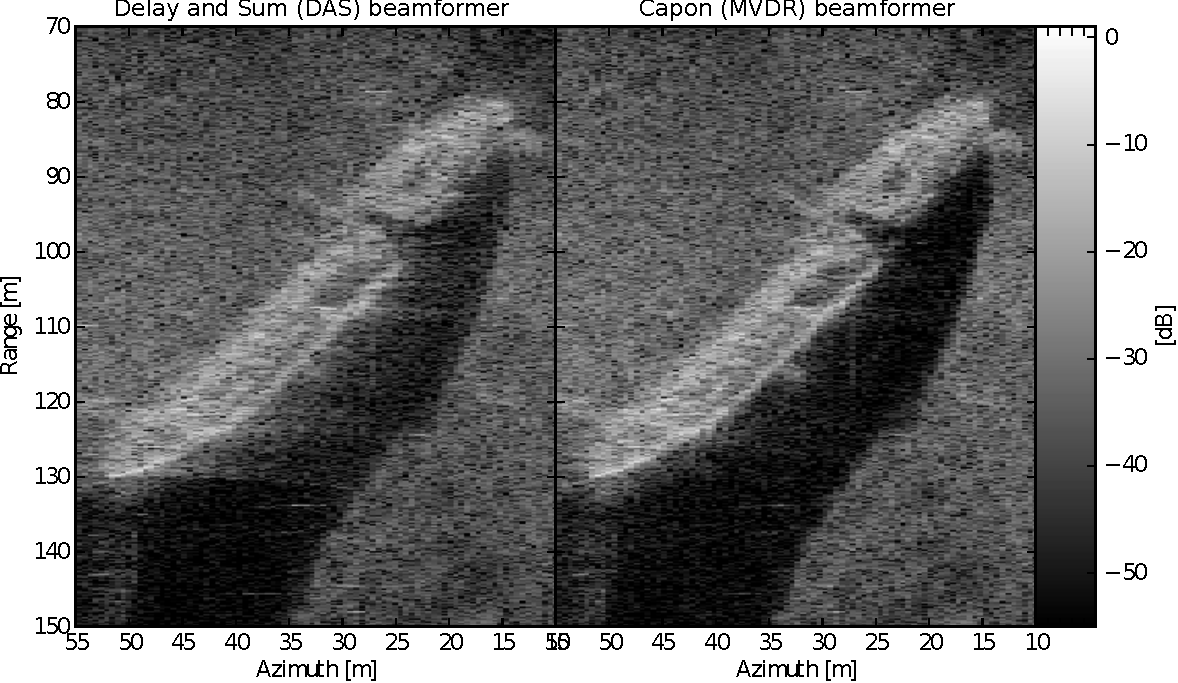
\includegraphics[width=\linewidth]{gfx/img_holmengraa.pdf}
\caption{HISAS sidescan sonar (SSS) image of the shipwreck Holmengraa.}\label{holmengraa}
\end{figure}


\section{Implementation}
The paradigm of \gls{GPU} computing is formalized as the execution of thousand of threads, where each thread runs a copy of a common function, also know as a kernel. Threads are organized in blocks, and blocks further into a grid of blocks. The threads index in this grid usually decides the data to be process and the instruction path to go along. A modern \gls{GPU} is an hardware architecture comprised of several hundred computing cores, each having access to a very limited amount of local memory an registers. This suggests that the algorithm should be decomposed into as many lightweight threads as possible. For a typical array configuration, using a single thread per pixel for Capon is not lightweight enough. Therefore, we seek to devise a way to decompose the methods presented in section \ref{methods}. In particular, the solutions we came up with for the different steps in the algorithm, listed in their natural order of execution, was:
\begin{enumerate}
\item \emph{Computing the spatial covariance matrix} $\eR[n]$ (equation \ref{spatialR}-\ref{finalR}). A group of threads are created that slide along the diagonals of $\eR$. In this way we can exploit the fact that entries on the diagonals overlaps across subarrays and time. 
%Finished threads can also wrap around and start on diagonals on the lower half triangular. 
In this way we process one row of $\eR$ per kernel iteration, and manage to keep the numbers of both data reads and writes at a minimum.
\item \emph{Computing} $\eRi[n]\1$ (from equation \ref{weights}). While intuition may suggest that this step is carried out by inverting $\eR$, it is better to solve the linear equation $\R\beta = \1$ for $\beta$ instead, which gives us $\beta = \eRi\1$ directly. We have tested various solvers for this task, both in-house and proprietary implementations, but achieved the best performance by using an unofficial batch solver from nVidia. Inverting $\eR$ is by far the most computationally intensive task, and a key area of focus for further improvements.
\item \emph{Computing the subarray weights} by substituting $\beta = \eRi[n]\1$ into equation \ref{weights}, $\vec w[n] = \frac{\beta}{\1\T\beta}$. A group of L threads per pixel was used to reduce shared memory pressure and to obtain coalesced reads and a minimum of writes. \emph{Finally we acquire the pixel value $z[n]$} by applying the weights to each data vector $\x_l[n]$, and sum them all up (as in equation \ref{z}). When applying weights, there are two approaches from an implementation point of view. The subarray data can, as here, be reduced to coincide in length with the subarray weights, or the weights can be extended to M in size and applied directly on $\x[n]$ and summed.  
\end{enumerate}
For the GPU, the largest bottleneck is the transfer of memory from CPU-side (Host) to the GPU-side (Device). In the upcoming results, Host to Device transfer are not taken into account. The reasoning behind this is the fact that Capon beamforming requires already delayed data. For efficiency, this should also be carried out on the GPU, leaving the challenging task of overcoming the limited Host-Device memory bandwidth to those who implement the delay part of delay-and-sum. 


TODO:
\begin{itemize}
\item Choice of robustification parameters $L,M,\Delta$ largely impacts what the ``optimal'' way of implementing Capon 
\item Introduce CUDA, or ditch it?
\item Doesn't sell well that we used nVidias solver, especially when that's the bottleneck in the design...
\end{itemize}

\newpage

\section{Results}

We have tested \gls{GPU} implementation of the \gls{MVDR} beamformer on experimental data from 32 element Kongsberg Maritime HISAS1030 sonar~\cite{Hansen2009}\todo{specify SAS somewhere here..}. The sonar was attached to the HUGIN \gls{AUV}, and the imaged object was the 1500 dwt oil tanker wreck Holmengraa (fig. \ref{holmengraa}). Holmengraa is roughly 68\,m long and 9\,m wide, and lies on a slanted seabed at 77\,m depth. The Capon image was created with the parameters $L=16$, $N_\text{avg}=3$, and $d=1\%$.

\begin{figure}[!t]
\centering
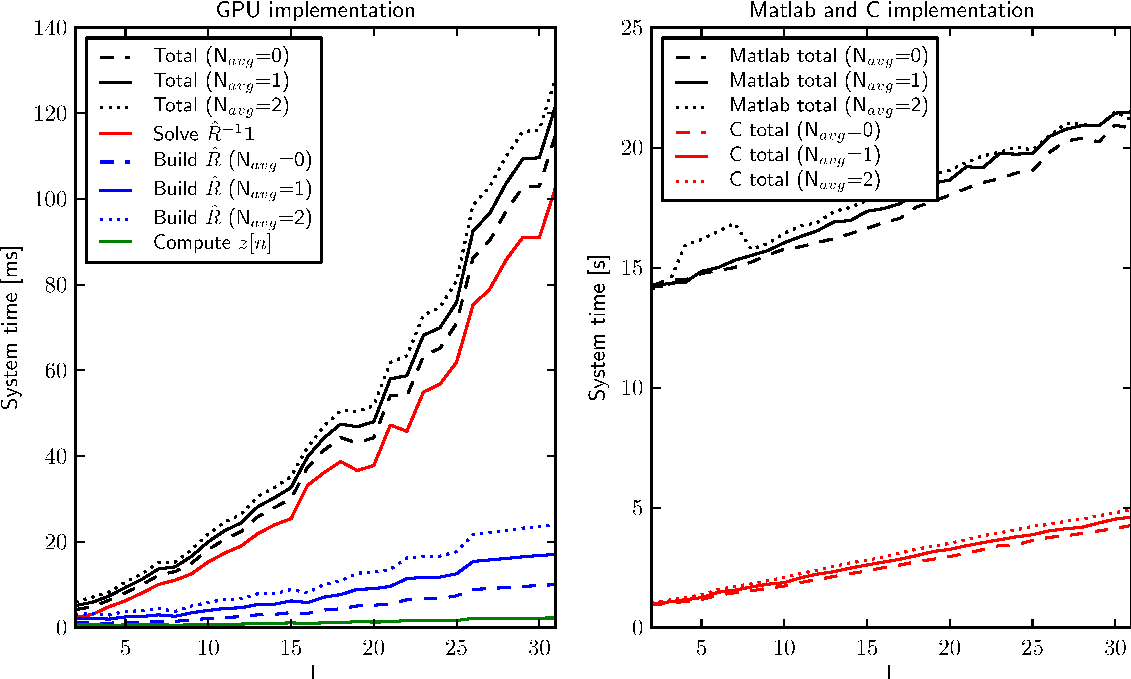
\includegraphics[width=\linewidth]{gfx/benchmark.pdf}
\caption{Capon benchmarks.}\label{benchmarks}
\end{figure}

Benchmarks\\
The test system was a quad-core Intel Xeon E5620, 64Gb of \gls{RAM}, and an nVidia Quadro 6000 card. This is a \gls{GPU} with 448 \gls{CUDA} cores and 6Gb of onboard \gls{RAM}, capable of roughly 1Tflops.


\section{Discussion}

\begin{itemize}
\item Relate Capon image to DAS image
\item Discuss the benchmarks
\item Need for speed: HUGIN 4 banks of 32 elements, can be processed faster than the ping repetition rate, with margins to spare.
\end{itemize}


\section{Conclusion}

\begin{itemize}
\item When to use what.
\end{itemize}



% A sidescan image of the 1500 dwt oil tanker wreck Holmengraa is shown in \Fig{holmengraa}.  depth~\cite{holmengraa}. The sidescan image was created using data from the HISAS 1030 sonar, which is rather unsuited for this purpose because of its large opening angle. This, and the fact that the wreck was imaged at a range of about 105\,m makes the image quality poor, but sufficient to compare our beamformers. 

% % In the Holmengraa image we note again that the LCA produces a cleaner shadow and better edge definition. The MV method performed almost identically to LCA in this case, and was omitted.
% 
% 
% 
% down to these cores and back to the \gls{CPU} is also when copying data to and from the \gls{GPU} are also rather high, so each core should be   performing calculations there, and copying the data back to the \gls{CPU}
% 
%  but in order to fully exploit this potential we must be aware of its limitations.  
% 
% When adapting an algorithm to a massively parallel hardware such as \glspl{GPU}, one must be familiar with its limitations in order to that the potential that lies within these chips can not be fully realised 
% 
% When trying to fit any algorithm to massively parallel hardware such as \glspl{GPU}, one must be careful to select a proper decomposition scheme for the device at hand. Modern \glspl{GPU} have several hundred computing cores, but only a limited amount of  are  various decomposition schemes should be contemplated before performing the implecareful decomposition of the 
% 
% 
% Let us first consider the \emph{computation of $\hat{\mat R}$}. Notice that when implementing the formula directly a lot of summations and multiplications will be repeated unnecessary. To illustrate this, consider for instance a case with $M=6$ sensors that are grouped into subarrays of length $L=3$ where all but one element overlap. Let us further assume that we need to average over 7 time samples, i.e. that $N_{\text{avg}} = 3$. 
% 
% These procedures are commutative, so the order in which we perform them does not matter. But for the sake of this example let us start by performing the time averaging. Assuming that $\vec x_i$ and $\vec x_j$ have a zero mean, a time averaged covariance coefficient $r_{ij}$ in $\hat{\mat R}$ may be obtained by (omitting the normalisation):
% \begin{align*}
% r_{ij}[n] &= \sumb{n'=n-N_{\text{avg}}}{n+N_{\text{avg}}} x_i[n']\,x_j[n'],
% \end{align*}
% which can be easily rewritten in a sliding window fashion
% \begin{align*}
% \hat r_{ij}[n] &= r_{ij}[n-1] - x_i[n\text{-}N_\text{avg}\text{-}1]\,x_j[n\text{-}N_\text{avg}\text{-}1]
%                          + x_i[n\text{+}N_\text{avg}]\,x_j[n\text{+}N_\text{avg}].
% \end{align*}
% Hence, whenever $N_\text{avg}>1$ the sliding window approach will demand less instructions at the expense of a slightly higher memory consumption. The next thing to realise is that not all $r_{ij}[n]$ need to be computed. Since $r_{ji} = r^*_{ij}$, and the subarrays only span $L$ elements, we only compute an upper triangular band of R (marked \Green{green})
% \begin{figure}[H]
% % \begin{narrow}{-3.5cm}{-3.5cm}
% 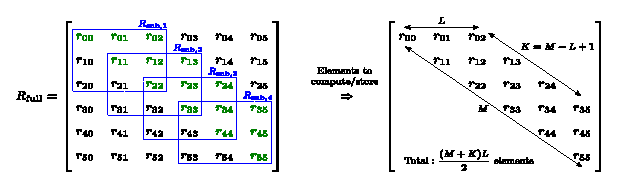
\includegraphics[width=\linewidth]{gfx/capon_build_R_full.eps}
% \caption{Building $\hat{\mat R}$: Symmetry and element coverage}\label{buildingRfull}
% % \end{narrow}
% \end{figure}
% The final step is to average all the subarray matrices to form $\hat{\mat R}$ by 
% {\renewcommand*{\arraystretch}{1.8}
% \begin{align*}
% \hat{\mat R}_\text{sub} &= {\color{Blue}\mat R_{\text{sub},1} + \mat R_{\text{sub},2} + \mat R_{\text{sub},3} + \mat R_{\text{sub},4}} \\
% &= \left[\;
% \begin{matrix}
% \color{Green}r_{00}+r_{11}+r_{22} & \color{Red}r_{01}+r_{12}+r_{23} & r_{02}+r_{13}+r_{24} \\
%                                        & \color{Green}r_{11}+r_{22}+r_{33} & \color{Red}r_{12}+r_{23}+r_{34} \\
%                                        &                                        & \color{Green}r_{22}+r_{33}+r_{44}
% \end{matrix}
% \;\right]
% \end{align*}}%
% Note that consecutive elements along the diagonals overlap on all but one covariance coefficient, hence a sliding window may also be used here. The subarray size $L$ is usually quite a bit larger than the time averaging window, so there is more to gain from implementing the sliding window here.\\\\
% 
% {\bf Method complexity:}\\
% \begin{tabular}{l l}
% No optimizations            & $2M^2\,(2\Navg+1)$ \\
% Banded symmetric            & $L(2M-L+1)\,(2\Navg+1)$ \\
% Sliding, banded, symmetric  & $1.5L(2M-L+1)$ \\
% \end{tabular}\\\\



% \subsubsection{Computing $\text{\raisebox{1.9pt}{$\vec\chi$}} = \hat{\mat R}\,\!^{-1}\vec a$}
% 
% There are two ways of finding $\text{\raisebox{1.9pt}{$\vec\chi$}} = \hat{\mat R}\,\!^{-1}\vec a$, either by solving the equation directly or by inverting $\hat{\mat R}$ first. Solving the equation is less computationally intensive than inverting $\hat{\mat R}$, and seems like the obvious choice. However, with iterative methods for updating $\eRi$ for each range pixel the situation is changed...
% 
% 
% \section{Results/Discussion}
% 
% 
% 
% 
% 
% \todopar{Case:
% \begin{itemize}
% \item JOE
% \item Sonar. Channel count up to 32/64 ish channels?
% \item Other articles evaluates Capon image quality, and some have shown that speedups can be achieved by reducing the complexity of the traditional Capon algorithm or by implementing specific versions on a GPU.
% \item This article compare a few promising ways to implement Capon in general, in light of general complexity and suitability for implementation on a CPU and GPU.
% \end{itemize}
% }
% 
% \begin{itemize}
% \item As briefly as possible, introduce beamforming.
% \item Adaptive beamformer's potential lies in its ability to suppress interference power
% \item Why adaptive beamformers struggle in active sonar systems. Correlated noise, robustification kills the adaptive potential. Quite computationally intensive. Constraints must be applied in one way or another - parameters must be tuned.
% \item The three main ways to implement Capon \cite{Capon1969} is \todo{not entirely true?}
% \begin{itemize}
% \item Traditional way: Build $\eR$ and solve $\w = \frac{\Ri\a}{\a\H\Ri\a}$. 
% \item Iterative methods: Woodbury, Conjugated gradients
% \item Beamspace
% \item LCA (or other methods, as reference)
% \end{itemize}
% \item Choice of robustification parameters $L,M,\Delta$ largely impacts what the ``optimal'' way of implementing Capon 
% \item In most imaging applications 
% Outline:
% \begin{itemize}
% \item Speeding up: Build $\eR$ and solve $\w = \frac{\Ri\a}{\a\H\Ri\a}$. 
% \item Iterative methods: Woodbury (Sherman Morrison), Conjugated gradients - show performance of GPU performance.
% \item Woodbury: Must take the average over many samples in space and time - lots of (small) outerproducts. Can be used if not a lot of averaging is required.
% \item Beamspace
% \item LCA (or other methods, as reference)
% \end{itemize}
% \end{itemize}
% 

% \ \\
% \IEEEPARstart{T}{o} form images from a modern phased array sonar system the received wavefield is usually recorded, and then postprocessed by a digital beamformer. The beamformer applies delays and weights to the sensor channels, the beamformer adjusts the arrays spatial response to focus at one pixel at a time.  such that signals emanating from regions of interest add constructively, while ensuring that noise and interference from other angles do not. 
% 
% The imaging capabilities of a modern phased array sonar system depend on physical attributes such element response and array geometry, the transmitted signal, as well as the beamforming method being used on transmission and reception. Beamforming is the concept of applying delays and weights to the sensors channels to steer the arrays response to points of interest. 

% 
% 
% Outline:
% \begin{itemize}
% \item Capon's resonse when applying robustification
% \item Choice of window functions makes little difference.
% \item Steering and mainlobewidths have outer bounds.
% \item Beamspace?
% \item Chosen window plots - what may they tell us? Variance intensity values when using various windows.
% \item Assymmetric windows?
% \end{itemize}
% 
% 
% \begin{align}
% z[n] = \sumb{m=0}{M-1} w_m[n]^*x_m[n-\Delta_m] = \w\H[n]\x[n-\Delta_m]
% \end{align}
% 
% 
% \section{Methods}
% 
% Basically, we are working with a practical implementation of the Capon beamformer that computes a set of weights $\vec w$ for every single sample $n$ by solving:
% \begin{gather*}
% \vec w[n] = \frac{\hat{\mat R}\,\!^{-1}[n]\vec a}{\vec a\H\hat{\mat R}\,\!^{-1}[n]\vec a} = \frac{\text{\raisebox{1.9pt}{$\vec\chi$}}[n]}{\vec a\H\text{\raisebox{1.9pt}{$\vec\chi$}}[n]}
% \end{gather*}%
% where
% % \newcommand\X{\text{\raisebox{2pt}{$\vec\chi$}}}
% \begin{gather*}
% \text{\raisebox{1.9pt}{$\vec\chi$}} = \hat{\mat R}\,\!^{-1}\vec a \qquad\qquad\text{is the solution to}\qquad\qquad \hat{\mat R}\text{\raisebox{1.9pt}{$\vec\chi$}} = \vec a.
% \end{gather*}

% 
% , and maximum suppression of while ensuring that the beamformer digitally  before each of the pixels are estimated one at a time. The resolution and contrast of such a system will depend on the systems spatial response, which ideally should be narrow  be very sharp in the desired direction its ability to achieve  fundamental principle of forming a sonar image is to record the received wavefield, 
% 
% image quality of a phased array sonar imaging systems depend on  the choice of weights to apply to each of the sensors are crucial. 
% 
% A modern phased array imaging system may be thought of as a spatial filter. To achieve the best possible performance, the 
% 
% resolution and contrast 
% 
% Adaptive beamformers have only recently been introduced in active sonar imaging. For a while they were considered unsuited for this purpose because the backscattered signal is largely correlated with the 
% 
% 
% 

%\begin{figure}[!t]
%\centering
%\includegraphics[width=2.5in]{myfigure}
% where an .eps filename suffix will be assumed under latex, 
% and a .pdf suffix will be assumed for pdflatex; or what has been declared
% via \DeclareGraphicsExtensions.
%\caption{Simulation Results}
%\label{fig_sim}
%\end{figure}


% An example of a double column floating figure using two subfigures.
% (The subfig.sty package must be loaded for this to work.)
% The subfigure \label commands are set within each subfloat command, the
% \label for the overall figure must come after \caption.
% \hfil must be used as a separator to get equal spacing.
% The subfigure.sty package works much the same way, except \subfigure is
% used instead of \subfloat.
%
% \begin{figure*}[!t]
% \centerline{\subfloat[Case I]\includegraphics[width=2.5in]{subfigcase1}%
% \label{fig_first_case}}
% \hfil
% \subfloat[Case II]{\includegraphics[width=2.5in]{subfigcase2}%
% \label{fig_second_case}}}
% \caption{Simulation results}
% \label{fig_sim}
% \end{figure*}
%
% Note that often IEEE papers with subfigures do not employ subfigure
% captions (using the optional argument to \subfloat), but instead will
% reference/describe all of them (a), (b), etc., within the main caption.


% An example of a floating table. Note that, for IEEE style tables, the 
% \caption command should come BEFORE the table. Table text will default to
% \footnotesize as IEEE normally uses this smaller font for tables.
% The \label must come after \caption as always.
%
%\begin{table}[!t]
%% increase table row spacing, adjust to taste
%\renewcommand{\arraystretch}{1.3}
% if using array.sty, it might be a good idea to tweak the value of
% \extrarowheight as needed to properly center the text within the cells
%\caption{An Example of a Table}
%\label{table_example}
%\centering
%% Some packages, such as MDW tools, offer better commands for making tables
%% than the plain LaTeX2e tabular which is used here.
%\begin{tabular}{|c||c|}
%\hline
%One & Two\\
%\hline
%Three & Four\\
%\hline
%\end{tabular}
%\end{table}


% Note that IEEE does not put floats in the very first column - or typically
% anywhere on the first page for that matter. Also, in-text middle ("here")
% positioning is not used. Most IEEE journals use top floats exclusively.
% However, Computer Society journals sometimes do use bottom floats - bear
% this in mind when choosing appropriate optional arguments for the
% figure/table environments.
% Note that, LaTeX2e, unlike IEEE journals, places footnotes above bottom
% floats. This can be corrected via the \fnbelowfloat command of the
% stfloats package.
% 
% 
% 
% \section{Conclusion}
% The conclusion goes here.
% 
% 
% 
% 
% 
% % if have a single appendix:
% %\appendix[Proof of the Zonklar Equations]
% % or
% %\appendix  % for no appendix heading
% % do not use \section anymore after \appendix, only \section*
% % is possibly needed
% 
% % use appendices with more than one appendix
% % then use \section to start each appendix
% % you must declare a \section before using any
% % \subsection or using \label (\appendices by itself
% % starts a section numbered zero.)
% %

%%%%%%%%%%%%%%%%%%                              ~~~~~~~~~~~~~~~~~~~~~~~~~~~~~~~~~~~~~~~~~~~~~~~~~~
% DOCUMENT APPENDICES %
%%%%%%%%%%%%%%%%%%                              ~~~~~~~~~~~~~~~~~~~~~~~~~~~~~~~~~~~~~~~~~~~~~~~~~~

% 
\section{Acknowledgments}

The authors would like to thank...


\bibliographystyle{./template/ecua}
\bibliography{../../Library/library}


\end{document}


